\chapter{Decision Trees}

\section{Classification}

Classification is a data mining task that assigns a class label to a record based on its attribute values.

{We start off with \textbf{training set} of records, each characterized by a tuple $(x,y)$,
where $x$ is the attribute set and $y$ is the class label
\begin{itemize}\ns
	\item $x$: attribute, predictor, independent variable, input
	\item $y$: class, response, dependent variable, output
\end{itemize}}

The goal of classification is to learn a function (often called ``\textbf{model}'') $f: X \rightarrow Y$ that maps each attribute set $x$ into one of the predefined class labels y.

The \textbf{goal} of classification is to accurately predict the class labels of \textbf{unseen records} (i.e., records not in the training set).\\
A test set is used to determine the accuracy of the model.
Usually, the given data set is divided into training and test sets,
with training set used to build the model and test set used to
validate it.

\begin{itemize}
	\item \textbf{Base classifier}: a classifier built from the training set
	      \begin{itemize}
		      \item Decision Tree based Methods
		      \item Rule-based Methods
		      \item Nearest-neighbor
		      \item Neural Networks
		      \item Deep Learning
		      \item Naïve Bayes and Bayesian Belief Networks
		      \item Support Vector Machines
	      \end{itemize}
	\item \textbf{Ensemble classifier}: a classifier that combines multiple base classifiers to improve accuracy
	      \begin{itemize}
		      \item Bagging
		      \item Boosting
		      \item Random Forests
	      \end{itemize}
\end{itemize}

\section{Classification with Decision Trees}
A decision tree is a flowchart-like tree structure, where each internal node denotes a test on an attribute, each branch represents the outcome of the test, and each leaf node holds a class label.

There are various algorithms to build decision trees, such as Hunt's algorithm (among the earliest ones), ID3, C4.5, CART, etc.

\subsection{Hunt's Algorithm}
Let $D_t$ be the set of training records at node $t$.
The general procedure of Hunt's algorithm is as follows:
\begin{itemize}
	\item If $D_t$ contains records that belong the same class $y_t$, then $t$ is a leaf node labeled as $y_t$
	\item If $D_t$ contains records that belong to more than one class, use an attribute test to split the data into smaller subsets. Recursively apply the procedure to each subset.
\end{itemize}

\subsubsection{Example: Building a Decision Tree Step-by-Step}

\begin{figure}[htbp]
      \centering
      \includegraphics{images/11/huntSteps.png}
      \caption{Hunt's algorithm steps applied to Table \ref{tab:example}}
      \label{fig:11/huntSteps}
\end{figure}

\begin{table}[h]
\centering
\begin{tabular}{|c|c|c|c|c|}
\hline
\rowcolor{blue!80}
\textcolor{white}{\textbf{ID}} & \textcolor{white}{\makecell{\textbf{Home}\\\textbf{Owner}}} & \textcolor{white}{\makecell{\textbf{Marital}\\\textbf{Status}}} & \textcolor{white}{\makecell{\textbf{Annual}\\\textbf{Income}}} & \textcolor{white}{\makecell{\textbf{Defaulted}\\\textbf{Borrower}}} \\
\hline
\rowcolor{gray!20}
1 & Yes & Single & 125K & \textcolor{red}{\textbf{No}} \\
\hline
2 & No & Married & 100K & \textcolor{red}{\textbf{No}} \\
\hline
\rowcolor{gray!20}
3 & No & Single & 70K & \textcolor{red}{\textbf{No}} \\
\hline
4 & Yes & Married & 120K & \textcolor{red}{\textbf{No}} \\
\hline
\rowcolor{gray!20}
5 & No & Divorced & 95K & \textcolor{red}{\textbf{Yes}} \\
\hline
6 & No & Married & 60K & \textcolor{red}{\textbf{No}} \\
\hline
\rowcolor{gray!20}
7 & Yes & Divorced & 220K & \textcolor{red}{\textbf{No}} \\
\hline
8 & No & Single & 85K & \textcolor{red}{\textbf{Yes}} \\
\hline
\rowcolor{gray!20}
9 & No & Married & 75K & \textcolor{red}{\textbf{No}} \\
\hline
10 & No & Single & 90K & \textcolor{red}{\textbf{Yes}} \\
\hline
\end{tabular}
\caption{Example dataset for classification}
\label{tab:example}
\end{table}


Using the dataset in Table \ref{tab:example}, we can illustrate how Hunt's algorithm builds a decision tree iteratively:

\textbf{Step (a):} The algorithm starts with all training records at the root node. The initial dataset contains 10 records with 7 instances of ``No'' and 3 instances of ``Yes'' for the Defaulted Borrower class. Since the node contains records from both classes, we need to split the data.

{\textbf{Step (b):} The algorithm selects \textit{Home Owner} as the first splitting attribute. This creates two branches:\ns
\begin{itemize}
	\item \textbf{Home Owner = Yes:} Contains 3 records, all with class label ``Defaulted = No'' (3,0). Since all records belong to the same class, this becomes a leaf node.
	\item \textbf{Home Owner = No:} Contains 7 records with 4 instances of ``No'' and 3 instances of ``Yes'' (4,3). Since this node contains mixed classes, further splitting is required.
\end{itemize}}

{\textbf{Step (c):} The algorithm continues by splitting the \textit{Home Owner = No} branch using \textit{Marital Status} as the splitting attribute:\ns
\begin{itemize}
	\item \textbf{Home Owner = No, Marital Status = Single or Divorced:} Contains 4 records with 1 instance of ``No'' and 3 instances of ``Yes'' (1,3). The majority class is ``Yes'', but the node is not pure.
	\item \textbf{Home Owner = No, Marital Status = Married:} Contains 3 records, all with class label ``Defaulted = No'' (3,0). This becomes a leaf node.
\end{itemize}}

{\textbf{Step (d):} The algorithm makes a final split on the remaining impure node (\textit{Home Owner = No, Marital Status = Single or Divorced}) using \textit{Annual Income} with threshold 80K:\ns
\begin{itemize}
	\item \textbf{Home Owner = No, Marital Status = Single/Divorced, Annual Income < 80K:} Contains 1 record with class ``Defaulted = No'' (1,0). This becomes a leaf node.
	\item \textbf{Home Owner = No, Marital Status = Single/Divorced, Annual Income $\geq$ 80K:} Contains 3 records with class ``Defaulted = Yes'' (0,3). This becomes a leaf node.
\end{itemize}}

At this point, all leaf nodes contain records from a single class (pure nodes), and the decision tree is complete. The tree can now be used to classify new instances by traversing from the root to a leaf based on the attribute values of the test record.




\subsubsection{Splitting Strategies}

When building decision trees, there are different strategies for splitting nodes based on categorical attributes:

\begin{figure}[htbp]
\centering

% Multi-way split
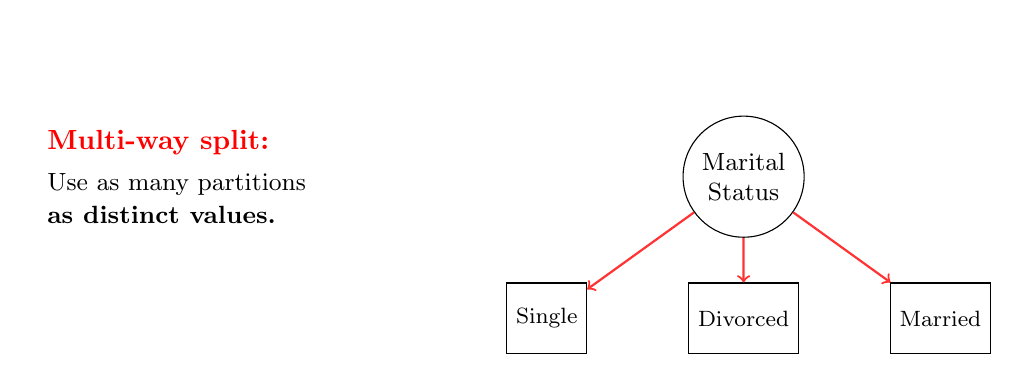
\begin{tikzpicture}[
    level distance=1.8cm,
    level 1/.style={sibling distance=2.5cm},
    every node/.style={circle, draw, align=center, minimum size=1.3cm, font=\small},
    edge from parent/.style={draw, ->, thick, red!80},
    leaf/.style={rectangle, draw=black, minimum size=0.9cm, font=\footnotesize}
]

\node {Marital\\Status}
    child {node[leaf] {Single}}
    child {node[leaf] {Divorced}}
    child {node[leaf] {Married}};

\node[draw=none, align=left, font=\normalsize\bfseries] at (-7.2, 0) {\textcolor{red}{Multi-way split:}\\[0.1cm] \normalfont\small Use as many partitions\\\small as distinct values.};

\end{tikzpicture}

\vspace{0.8cm}

% Binary splits
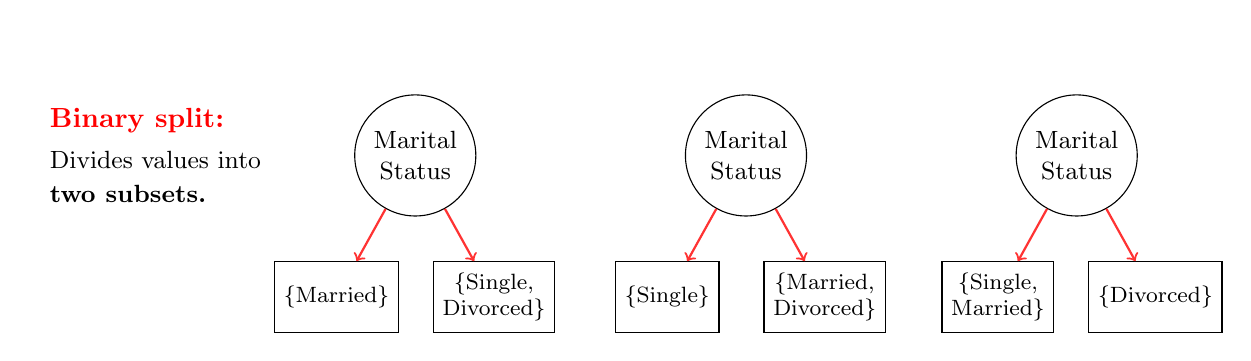
\begin{tikzpicture}[
    level distance=1.8cm,
    level 1/.style={sibling distance=2cm},
    every node/.style={circle, draw, align=center, minimum size=1.3cm, font=\small},
    edge from parent/.style={draw, ->, thick, red!80},
    leaf/.style={rectangle, draw=black, minimum size=0.9cm, font=\footnotesize}
]

% Binary split - example 1
\node (ms1) at (0,0) {Marital\\Status}
    child {node[leaf] {\{Married\}}}
    child {node[leaf] {\{Single,\\Divorced\}}};

% Binary split - example 2
\node (ms2) at (4.2,0) {Marital\\Status}
    child {node[leaf] {\{Single\}}}
    child {node[leaf] {\{Married,\\Divorced\}}};

% Binary split - example 3
\node (ms3) at (8.4,0) {Marital\\Status}
    child {node[leaf] {\{Single,\\Married\}}}
    child {node[leaf] {\{Divorced\}}};

\node[draw=none, align=left, font=\normalsize\bfseries] at (-3.3, 0) {\textcolor{red}{Binary split:}\\[0.1cm] \normalfont\small Divides values into\\\small two subsets.};

\end{tikzpicture}

\caption{Splitting strategies for categorical attributes: Multi-way vs Binary splits}
\label{fig:splitting-strategies}
\end{figure}

\textbf{Multi-way split:} Creates as many child nodes as there are distinct values in the attribute. For example, splitting on Marital Status with three values (Single, Divorced, Married) creates three branches. This approach is intuitive but can lead to data fragmentation, especially when attributes have many distinct values.

\textbf{Binary split:} Divides the attribute values into two subsets, creating only two child nodes. There are multiple ways to partition the values (e.g., \{Married\} vs \{Single, Divorced\}, or \{Single\} vs \{Married, Divorced\}, etc.). Binary splits are preferred in algorithms like CART as they create more balanced trees and are computationally more efficient, though they may require more splits to achieve the same separation.

% example table

\subsubsection{Continuous attributes}
There are two main approaches to handle continuous attributes in decision trees:
\begin{itemize}
      \item \textbf{Discretization} to form an ordinal categorical attribute based on a set of \textbf{intervals}.
      Such intervals may be determined using domain knowledge or algorithms like equal-width or equal-frequency binning (percentiles), or clustering.\\
      The discretization may be static, so performed only once at the beginning of the tree construction, or dynamic, so performed at each node during tree construction.
      \item \textbf{Binary splits} based on thresholding, e.g., Income $\leq$ 100K vs Income $>$ 100K.\\
      All possible splits should be considered to find the best threshold that optimizes a certain criterion (e.g., information gain, Gini index, etc.).
      This may result in an intensive computation.
\end{itemize}

\begin{figure}[htbp]
\centering

% Binary split
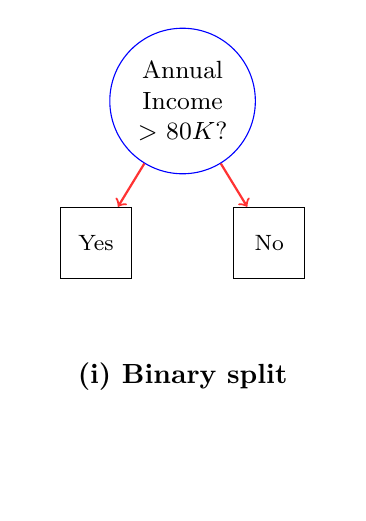
\begin{tikzpicture}[
    level distance=1.8cm,
    level 1/.style={sibling distance=2.2cm},
    every node/.style={circle, draw=blue, align=center, minimum size=1.3cm, font=\small},
    edge from parent/.style={draw, ->, thick, red!80},
    leaf/.style={rectangle, draw=black, minimum size=0.9cm, font=\footnotesize}
]

\node {Annual\\Income\\$>$ $80K$?}
    child {node[leaf] {Yes} edge from parent node[left, draw=none, font=\small] {}}
    child {node[leaf] {No} edge from parent node[right, draw=none, font=\small] {}};

\node[draw=none, align=center, font=\normalsize\bfseries] at (0, -3.5) {(i) Binary split};

\end{tikzpicture}
\hspace{2cm}
% Multi-way split
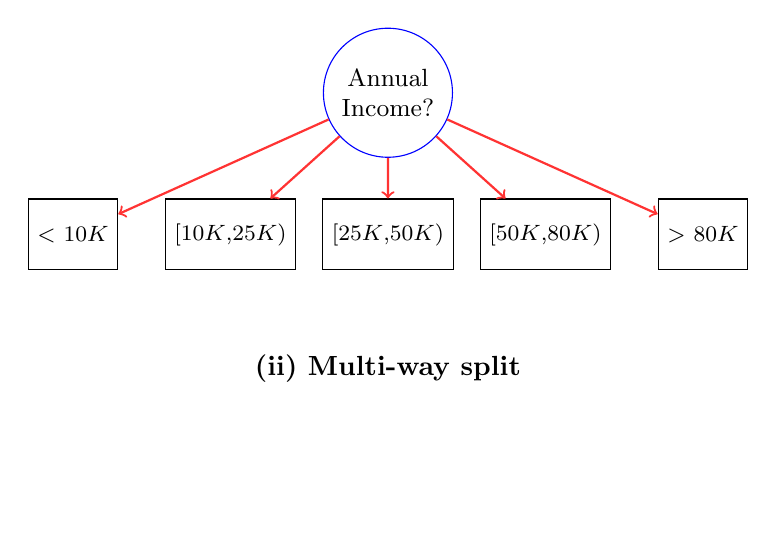
\begin{tikzpicture}[
    level distance=1.8cm,
    level 1/.style={sibling distance=2cm},
    every node/.style={circle, draw=blue, align=center, minimum size=1.3cm, font=\small},
    edge from parent/.style={draw, ->, thick, red!80},
    leaf/.style={rectangle, draw=black, minimum size=0.9cm, font=\footnotesize}
]

\node {Annual\\Income?}
    child {node[leaf] {$<$ $10K$} edge from parent node[left, draw=none, font=\tiny, pos=0.7] {}}
    child {node[leaf] {[$10K$,$25K$)} edge from parent node[left, draw=none, font=\tiny] {}}
    child {node[leaf] {[$25K$,$50K$)} edge from parent node[draw=none, font=\tiny] {}}
    child {node[leaf] {[$50K$,$80K$)} edge from parent node[right, draw=none, font=\tiny] {}}
    child {node[leaf] {$>$ $80K$} edge from parent node[right, draw=none, font=\tiny, pos=0.7] {}};

\node[draw=none, align=center, font=\normalsize\bfseries] at (0, -3.5) {(ii) Multi-way split};

\end{tikzpicture}

\caption{Splitting strategies for continuous attributes}
\label{fig:continuous-splitting}
\end{figure}

\newpage
\subsubsection{Choosing the best split}
Nodes with purer homogeneous class distributions are preferred.
\ul{To measure the \textbf{impurity} of a node}, we can use metrics such as \textbf{Gini Index},\textbf{Information Gain}(?), \textbf{Entropy} or \textbf{Misclassification error}.

\begin{align*}
      \textit{given:} \quad & p(i|t) = \text{proportion of records in node } t \text{ that belong to class } i\\
      \quad & \text{relative frequency of class \textit{i} at node \textit{t}}\\
\textbf{Gini Index:} \quad & Gini(t) = 1 - \sum_{i=1}^{c} p(i|t)^2 \\
\textbf{Entropy:} \quad & Entropy(t) = - \sum_{i=1}^{c} p(i|t) \log_2 p(i|t) \\
\textbf{Misclassification Error:} \quad & ME(t) = 1 - \max_{i} p(i|t)
\end{align*}

Practically, we compute the chosen impurity measure $P$ before splitting attributes, and then we compute it again ($M$) after the split for each child node.
$M$ is usually a weighted average of the impurity measures of the child nodes.

At this point we may choose the attribute test condition that produces the highest gain $G = P - M$, or, equivalently, the lowest impurity measure after splitting ($M$).
% attribute $A$ is selected for splitting that maximizes the impurity reduction: 

\subsection{Gini Index}

\subsubsection{Gini Index Examples}

The following examples illustrate how the Gini Index measures node impurity:

\begin{table}[h]
\centering
\begin{tabular}{|c|c|}
\hline
\textbf{C1} & \textbf{0} \\
\hline
\textbf{C2} & \textbf{6} \\
\hline
\end{tabular}
\quad
\begin{tabular}{l}
$P(C1) = 0/6 = 0$ \quad $P(C2) = 6/6 = 1$ \\[0.3cm]
$Gini = 1 - P(C1)^2 - P(C2)^2 = 1 - 0 - 1 = 0$
\end{tabular}
\end{table}

This represents a \textbf{pure node} where all instances belong to class C2. The Gini Index is 0, indicating no impurity.

\begin{table}[h]
\centering
\begin{tabular}{|c|c|}
\hline
\textbf{C1} & \textbf{1} \\
\hline
\textbf{C2} & \textbf{5} \\
\hline
\end{tabular}
\quad
\begin{tabular}{l}
$P(C1) = 1/6$ \quad $P(C2) = 5/6$ \\[0.3cm]
$Gini = 1 - (1/6)^2 - (5/6)^2 = 0.278$
\end{tabular}
\end{table}

This node has low impurity with most instances belonging to C2.

\begin{table}[h]
\centering
\begin{tabular}{|c|c|}
\hline
\textbf{C1} & \textbf{2} \\
\hline
\textbf{C2} & \textbf{4} \\
\hline
\end{tabular}
\quad
\begin{tabular}{l}
$P(C1) = 2/6$ \quad $P(C2) = 4/6$ \\[0.3cm]
$Gini = 1 - (2/6)^2 - (4/6)^2 = 0.444$
\end{tabular}
\end{table}

This node has higher impurity with a less uniform distribution. Note that the Gini Index reaches its maximum value of 0.5 (for two classes) when the distribution is perfectly balanced, e.g., $P(C1) = P(C2) = 0.5$. 

\subsubsection{Gini for a collection of nodes}

To compute the Gini Index for a collection of nodes after a split, we use a weighted average based on the number of instances in each child node.
\[
GINI_{split} = \sum_{i=1}^{k} \frac{n_i}{n} Gini(i)
\]
where:
\begin{itemize}
      \item $k$: number of child nodes after the split
      \item $n_i$: number of instances in child node $i$
      \item $n$: total number of instances in the parent node before the split
      \item $Gini(i)$: Gini Index of child node $i$
\end{itemize}

\note{Gini index is used in decision tree algorithms such as CART, SLIQ, SPRINT}

\note{There are some slides concerning optimizations on how the Gini index is computed when dealing with continuous attributes. These optimizations are not included here for brevity. By the way, they probably are already included in some Python library implementing decision trees \smiley .}

\paragraph{Entropy}
Entropy is another impurity measure used in decision trees, particularly in the ID3 and C4.5 algorithms. It quantifies the uncertainty or randomness in the class distribution of a node.\\
It is pretty similar to Gini index, but it tends to be more sensitive to changes in the class distribution.
For both of them, the lower the value, the purer the node.

\framedt{Note impurity limitations}{
      Node impurity measures tend to prefer splits that result in large number of partitions, each being small but pure.
      This may lead to overfitting, as the model captures noise in the training data rather than the underlying patterns.

      To mitigate this, we may consider also the number of child nodes created by a split when choosing the best attribute to split on. Or, as it happens in CART, we may use binary splits only, leading to have at most two child nodes per split.
}

\subsubsection{Comparing measures}
\begin{figure}[htbp]
      \centering
      \includegraphics{images/11/measures.png}
      \caption{Comparing Entropy, Gini and Misclassification error}
      \label{fig:11/measures}
\end{figure}

The image displays a 2-class problem. We can easily see that there is consistency among the three measures: they all reach their minimum (0) when the node is pure (i.e., all instances belong to one class) and their maximum when the classes are evenly distributed (i.e., $P(C1) = P(C2) = 0.5$).
Furthermore, if a node $N_1$ has lower entropy than node, $N_2$, then the Gini index and error rate of $N_1$, will also be lower than that of $N_2$

In some cases Gini may get better, but the misclassification error may stay exactly the same.

\section{Decision Trees Wrap Up}

\begin{itemize}
	\item Easy to interpret for small-sized trees
	\item Accuracy is comparable to other classification techniques for many simple data sets
	\item Robust to noise (especially when methods to avoid overfitting are employed)
	\item Can easily handle redundant or irrelevant attributes
	\begin{itemize}
            \item \textbf{Redundant} attributes: provide no additional information because they are highly correlated with other attributes
            \item \textbf{Irrelevant} attributes: provide no useful information for predicting the target class
      \end{itemize}
	\item Inexpensive to construct
      \item Extremely fast at classifying unknown record
	\begin{itemize}
            \item Construction cost: $O(M N log N)$ having $M$ attributes and $N$ records
            \item Testing cost: $O(\log N) = O(w)$ per record, where $w$ is the depth of the tree
      \end{itemize}
	\item Handle Missing Values
\end{itemize}

\begin{figure}[htbp]
      \centering
      \includegraphics{images/11/nodesComparison.png}
      \caption{The model on the right with 50 nodes probably overfits the data. This may lead to a high error rate on a test set}
      \label{fig:11/nodesComparison}
\end{figure}

\begin{figure}[htbp]
      \centering
      \includegraphics{images/11/underoverfit.png}
      \caption{Underfitting and overfitting}
      \label{fig:11/underoverfit}
\end{figure}

\section{Model selection}
Divide training data into two parts: a  \textbf{Training set} used for model building and a \textbf{Validation set} used for estimating generalization error.

Note that the validation set is not the same as the test set.
This is because the test set is used only at the very end to get an unbiased estimate of the generalization error.

This is a nice way to avoid overfitting, but the drawback is that there is less data available for training.


\begin{definition}
   [Occam's Razor]
   Given two models of similar generalization errors, one should prefer the simpler model over the more complex model.

   This is due to a complex model having a greater chance of being fitted accidentally by errors in data
\end{definition}

Occam's Razor suggests to include a penalty for model complexity in the estimate of generalization error.


\subsection{Evaluating Trees}
\begin{definition}
   [Pessimistic Error Estimate of decision tree T]
   
   Pessimistic Error Estimate of decision tree T with $k$ leaf nodes:

   \[err_{gen}(T) = err(T) + \Omega \times \frac{k}{N_{train}}\]
   \begin{itemize}
   	\item $err(T)$: error rate on all training records
   	\item $\Omega$: Relative cost of adding a leaf node
   	\item $k$: number of leaf nodes
   	\item $N_{train}$: total number of training record
   \end{itemize}
\end{definition}

\textbf{Minimum Description Length} (MDL) is another way to implement Occam's Razor.

\begin{definition}
   [Minimum Description Length]
   
   The best model is the one that minimizes the total description length:

   \[DL(Model) + DL(Data | Model)\]

   where:
   \begin{itemize}
   	\item $DL(Model)$: number of bits to describe the model
   	\item $DL(Data | Model)$: number of bits to describe the data when the model is known
   \end{itemize}
\end{definition}

\subsubsection{Estimating Statistical Bounds}
We can apply a statistical correction to the training error rate of the model that is indicative of its model complexity.

Doing so, we can obtain a statistical upper bound on the true error rate of the model.

To compute this statistical bound, we need the probability distribution of the training error, which can be either available from data or assumed.

In decision trees, the number of errors committed by a leaf node can be assumed to follow a \textbf{binomial distribution}. This is because:
\begin{itemize}
    \item Each instance in the leaf is classified as either correct or incorrect (binary outcome)
    \item We assume instances are independent
    \item The probability of error is constant for all instances in the leaf
\end{itemize}

Given a leaf node with $N$ instances and observed error rate $e$, we can compute a corrected error estimate $e'(N, e, \alpha)$ using the binomial confidence interval:

\[e'(N,e,\alpha) = \frac{e + \frac{z_{\alpha/2}^2}{2N} + z_{\alpha/2}\sqrt{\frac{e(1-e)}{N} + \frac{z_{\alpha/2}^2}{4N^2}}}{1 + \frac{z_{\alpha/2}^2}{N}}\]

where $z_{\alpha/2}$ is the critical value from the standard normal distribution at confidence level $\alpha$ (e.g., $z_{0.125} \approx 1.15$ for $\alpha = 0.25$).

The total generalized error for a tree $T$ is then:
\[e'(T) = \sum_{\text{leaves } L} N_L \times e'(N_L, e_L, \alpha)\]

This statistical correction penalizes small leaf nodes (which have higher uncertainty) and helps decide whether a split actually improves the model or just fits noise in the training data.

\subsubsection{Address overfitting}
\begin{itemize}
	\item Pre-pruning: stop growing the tree earlier
	      \begin{itemize}
		      \item Typical stopping conditions for a node are:
		            \begin{itemize}
			            \item Stop if all instances belong to the same class
			            \item Stop if all the attribute values are the same
		            \end{itemize}
		      \item More restrictive conditions:
		            \begin{itemize}
			            \item Stop if number of instances is less than some user-specified threshold
			            \item Stop if expanding the current node does not improve impurity measures (e.g., Gini or information gain).
			            \item Stop if estimated generalization error falls below certain threshold
		            \end{itemize}
	      \end{itemize}
	\item Post-pruning: grow the full tree, then remove nodes that do not help, following a bottom-up approach
	      % \begin{itemize}
	      %    \item Typical post-pruning methods:
	      %          \begin{itemize}
	      %             \item Reduced-error pruning: remove a node if the estimated generalization error of the subtree is higher than that of the node
	      %             \item Cost-complexity pruning: remove a node if the cost-complexity measure (e.g., MDL) of the subtree is higher than that of the node
	      %          \end{itemize}
	      % \end{itemize}\
	      \begin{itemize}
		      \item If generalization error improves after trimming, replace sub-tree by a leaf node.
		      \item Class label of leaf node is determined from majority class of instances in the sub-tree
		      \item Can use MDL for post-pruning
	      \end{itemize}
\end{itemize}

\subsubsection{Observations}

The number of possible decision trees can be very large, many decision tree algorithms employ a heuristic-based approach to guide their search in the vast hypothesis space.\\
That is \ul{\textbf{splitting} the records based on an attribute test that optimizes a certain criterion} (e.g., information gain, Gini index, etc.) at each node.

\coolquote{
      But then, how should training records be split at each node?\\
      And, how should the splitting procedure stop?
}{}

We need a method to \ul{specify a \textbf{test condition}} and a measure to evaluate the quality of a split, as well as a stopping criterion to prevent overfitting, which could be that if all records belong to the same class or if further splitting does not improve the model significantly.

\subsection{Test conditions}
Defining the test conditions to split the attributes depends on the type of attributes, whether they are categorical, binary, nominal, or continuous.



\section{Model Selection}

\subsection{Metrics for Performance evaluation}

To evaluate the performance of a classification model we must focus on the predictive capability of a model.
Rather than how fast it takes to classify or build models, scalability, etc.

We exploit a \textbf{confusion matrix} to evaluate the performance of a classification model, built like the following:

% // TODO
The most widely used metric based on the matrix is the \textbf{accuracy}.
\[
Accuracy = \frac{TP + TN}{TP + TN + FP + FN}
\]

Note that accuracy may be misleading when dealing with imbalanced classes.
Consider a dataset where 95\% of instances belong to class A and only 5\% to class B. A model that always predicts class A will have an accuracy of 95\%, but it fails to identify any instances of class B.

Another metric is $C(i|j)$, the \textbf{cost of erroneously classifying} an instance of class $j$ as class $i$.

We have also:
\begin{itemize}
   \item \textbf{Precision}:
         \[
         Precision = \frac{TP}{TP + FP}
         \]
   \item \textbf{Recall}:
         \[
         Recall = \frac{TP}{TP + FN}
         \]
   \item \textbf{F-measure}:
         \[
         F1 = 2 \times \frac{Precision \times Recall}{Precision + Recall}
         \]
   \item \textbf{Weighted accuracy}:
         \[
         Weighted\ Accuracy = \frac{TP + TN}{TP + TN + \beta \times FP + (1 - \beta) \times FN}
         \]
         or
         \[
         Weighted\ Accuracy = \frac{w_1\cdot TP + w_2\cdot TN}{w_1\cdot TP + w_2\cdot TN + w_3\cdot FP + w_4\cdot FN}
         \]
         where $\beta$ is a user-defined parameter that adjusts the weight of false positives and false negatives.
\end{itemize}

\section{Methods for Performance evaluated}

% // TODO

\section{Methods for Model Comparison}

To compare two models, we can use statistical tests to determine if the observed differences in performance are significant or due to random chance.

Comparing models is key when tuning hyperparameters, selecting features, or choosing between different algorithms.

\subsection{ROC - Receiver Operating Characteristic}

ROC curves plot the true positive rate (TPR) against the false positive rate (FPR) at various threshold settings.\\
The area under the ROC curve (AUC) provides a single measure of overall model performance.\\
Every point on the ROC curve represents the performance of each classifier, each having different trade-off between sensitivity and specificity.

% // TODO

\subsection{Significance Testing}

Given two models:
\begin{itemize}
	\item Model M1: $accuracy = 85\%$, tested on 30 instances
	\item Model M2: $accuracy = 75\%$, tested on 5000 instances
\end{itemize}

Is M1 really better than M2? 
Can the difference in performance measure be explained as a result of random fluctuations in the test set?\\
We can use significance testing to answer these questions.


\subsubsection{Confidence Interval for accuracy}
We can determine a confidence interval for accuracy, in order to estimate the range within which the true accuracy of the model lies, with a certain level of confidence.